\achapter{36}{The Gram-Schmidt Process in Inner Product Spaces} \label{sec:gram_schmidt_ips}

\vspace*{-17 pt}
\framebox{
\parbox{\dimexpr\linewidth-3\fboxsep-3\fboxrule}
{\begin{fqs}
\item What is the Gram-Schmidt process and why is it useful? 
\end{fqs}}}% \hspace*{3 pt}}

\vspace*{13 pt}

\csection{Application: Gaussian Quadrature}

Since integration of functions is difficult, approximation techniques for definite integrals are very important. In calculus we are introduced to various methods, e.g., the midpoint, trapezoid, and Simpson's rule,  for approximating definite integrals. These methods divide the interval of integration into subintervals and then use values of the integrand at the endpoints to approximate the integral. These are useful methods when approximating integrals from tabulated data, but there are better methods for other types of integrands. If we make judicious choices in the points we use to evaluate the integrand, we can obtain more accurate results with less work. One such method is Gaussian quadrature (which, for example, is widely used in solving problems of radiation heat transfer in direct integration of the equation of transfer of radiation over space), which we explore later in this section. This method utilizes the Gram-Schmidt process to produce orthogonal polynomials.

\csection{Introduction}

We have seen that orthogonal bases make computations very convenient, and the Gram-Schmidt process allowed us to create orthogonal bases in $\R^n$ using the dot product as inner product. In this section we will see how the Gram-Schmidt process works in any inner product space.  


\csection{The Gram-Schmidt Process using Inner Products}

Our goal is to understand how the Gram-Schmidt process works in any inner product space. 

\begin{pa} \label{pa:6_d_2}  Let $p_1(t) = t$, $p_2(t) = 1+t+t^2$, and $p_3(t) = t^3$ in $\pol_3$. Let $\CB = \{p_1(t), p_2(t), p_3(t)\}$ and let $W= \Span \ \CB$. Throughout this activity, use the inner product on $\pol_3$ defined by 
\[\langle p(t), q(t) \rangle = \int_{-1}^1 p(t)q(t) \, dt.\]
We want to construct an orthogonal basis $\CC = \{q_1(t), q_2(t), q_3(t)\}$ from $\CB$ so that $\Span \ \CC = \Span \ \CB$. To begin, we start by letting $q_1(t) = p_1(t)$. 
	\be
	\item Now we want to find a polynomial in $W$ that is orthogonal to $q_1(t)$. Let $W_1 = \Span\{q_1(t)\}$. Explain why $q_2(t) = \proj_{\perp W_1} p_2(t)$ is in $W$ and is orthogonal to $q_1(t)$. Then calculate the polynomial $q_2(t)$.  


	\item Next we need to find a third polynomial $q_3(t)$ that is in $W$ and is orthogonal to both $q_1(t)$ and $q_2(t)$. Let $W_2 = \Span \{q_1(t), q_2(t)\}$. Explain why $q_3(t) = \proj_{\perp W_2} p_3(t)$ is in $W$ and is orthogonal to both $q_1(t)$ and $q_2(t)$. Then calculate the polynomial $q_3(t)$.  

	\item Explain why the set $\{q_1(t), q_2(t), q_3(t)\}$ is an orthogonal basis for $W$. 


	\ee
	
\end{pa}

Preview Activity \ref{pa:6_d_2} shows the first steps of the Gram-Schmidt process to construct an orthogonal basis from any basis of an inner product space.  To understand how the process works in general, let $\{\vv_1, \vv_2, \ldots, \vv_m\}$ be a basis for a subspace $W$ of an inner product space $V$. Let $\vw_1 = \vv_1$ and let $W_1 = \Span\{\vw_1\}$. Since $\vw_1 = \vv_1$ we have that $W_1 = \Span\{\vw_1\} = \Span\{\vv_1\}$. Now consider the subspace 
\[W_2 = \Span\{\vv_1, \vv_2\}\]
of $W$. The vectors $\vv_1 = \vw_1$ and $\vv_2$ are possibly not orthogonal, but we know the orthogonal projection of $\vv_2$ onto $W_1^{\perp}$ is orthogonal to $\vw_1$. Let
\[\vw_2 = \proj_{\perp W_1} \vv_2 = \vv_2 -  \frac{\langle \vv_2, \vw_1 \rangle}{\langle \vw_1, \vw_1 \rangle} \vw_1.\]
Then $\{\vw_1, \vw_2\}$ is an orthogonal set. Note that $\vw_1 = \vv_1 \neq \vzero$, and the fact that $\vv_2 \notin W_1$ implies that $\vw_2 \neq \vzero$. So the set $\{\vw_1, \vw_2\}$ is linearly independent, being a set of non-zero orthogonal vectors. Now the question is whether $\Span\{\vw_1,\vw_2\} = \Span\{\vv_1,\vv_2\}$. Note that $\vw_2$ is a linear combination of $\vv_1$ and $\vv_2$, so $\vw_2$ is in $\Span\{\vv_1,\vv_2\}$. Since $\Span\{\vw_1,\vw_2\}$ is a 2-dimensional subspace of the 2-dimensional space $W_2$, it must be true that $\Span\{\vw_1,\vw_2\} = W_2 = \Span\{\vv_1,\vv_2\}$.

Now we take the next step, adding $\vv_3$ into the mix. Let 
\[W_3 = \Span\{\vv_1,\vv_2,\vv_3\} = \Span\{\vw_1, \vw_2, \vv_3\}.\] 
The vector
\[\vw_3 = \proj_{\perp W_2} \vv_3 = \vv_3 - \frac{\langle \vv_3, \vw_1 \rangle}{\langle \vw_1, \vw_1 \rangle} \vw_1 - \frac{\langle \vv_3, \vw_2 \rangle}{\langle \vw_2, \vw_2 \rangle} \vw_2\]
is orthogonal to both $\vw_1$ and $\vw_2$ and, by construction, $\vw_3$ is a linear combination of $\vv_1$, $\vv_2$, and $\vv_3$. So $\vw_3$ is in $W_3$. The fact that $\vv_3 \notin W_2$ implies that $\vw_3 \neq \vzero$ and $\{\vw_1, \vw_2, \vw_3\}$ is a linearly independent set. Since $\Span\{\vw_1, \vw_2, \vw_3\}$ is a 3-dimensional subspace of the 3-dimensional space $W_3$, we conclude that $\Span\{\vw_1, \vw_2, \vw_3\}$ equals $\Span\{\vv_1,\vv_2,\vv_3\}$.

We continue inductively in this same manner. If we have constructed a set $\{\vw_1$, $\vw_2$, $\vw_3$, $\ldots$, $\vw_{k-1}\}$ of $k-1$ orthogonal vectors such that \[\Span\{\vw_1, \vw_2, \vw_3, \ldots, \vw_{k-1}\} = \Span\{\vv_1,\vv_2,\vv_3, \ldots, \vv_{k-1}\},\]
then we let
\begin{align*}
\vw_{k} &= \proj_{\perp W_{k-1}} \vv_k \\
	&= \vv_k - \ds \frac{\langle \vv_k, \vw_1 \rangle}{\langle \vw_1, \vw_1 \rangle} \vw_1 - \frac{\langle \vv_k, \vw_2 \rangle}{\langle \vw_2, \vw_2 \rangle} \vw_2 - \cdots - \frac{\langle \vv_k, \vw_{k-1} \rangle}{\langle \vw_{k-1}, \vw_{k-1} \rangle} \vw_{k-1},
\end{align*}
where 
\[W_{k-1} = \Span\{\vw_1, \vw_2, \vw_3, \ldots, \vw_{k-1}\}.\]
We know that $\vw_k$ is orthogonal to $\vw_1$, $\vw_2$, $\ldots$, $\vw_{k-1}$. Since $\vw_1$, $\vw_2$, $\ldots$, $\vw_{k-1}$, and $\vv_k$ are all in $W_k = \Span\{\vv_1, \vv_2, \ldots, \vv_k\}$ we see that $\vw_k$ is also in $W_k$. Since $\vv_k \notin W_{k-1}$ implies that $\vw_k \neq \vzero$ and $\{\vw_1, \vw_2, \ldots, \vw_k\}$ is a linearly independent set. Then $\Span\{\vw_1, \vw_2, \vw_3, \ldots, \vw_{k}\}$ is a $k$-dimensional subspace of the $k$-dimensional space $W_k$, so it follows that 
\[\Span\{\vw_1, \vw_2, \vw_3, \ldots, \vw_{k}\} = W_k = \Span\{\vv_1,\vv_2,\vv_3, \ldots, \vv_{k}\}.\] 
This process will end when we have an orthogonal set $\{\vw_1$, $\vw_2$, $\vw_3$, $\ldots$, $\vw_{m}\}$ with $\Span\{\vw_1$, $\vw_2$, $\vw_3$, $\ldots$, $\vw_{m}\}$ = $W$.

We summarize the process in the following theorem.

\begin{theorem}[The Gram-Schmidt Process]\label{thm:6_d_Gram_Schmidt_ips}\index{Gram-Schmidt Process!in an inner product space} Let $\{\vv_1, \vv_2, \ldots, \vv_m\}$ be a basis for a subspace $W$ of an inner product space $V$. The set $\{\vw_1, \vw_2, \vw_3, \ldots, \vw_{m}\}$ defined by
\begin{itemize}
\item $\vw_1 = \vv_1$,
\item $\vw_2 = \vv_2 - \ds \frac{\langle \vv_2, \vw_1 \rangle}{\langle \vw_1, \vw_1 \rangle} \vw_1$,
\item $\vw_3 =  \vv_3 - \ds \frac{\langle \vv_3, \vw_1 \rangle}{\langle \vw_1, \vw_1 \rangle} \vw_1 - \frac{\langle \vv_3, \vw_2 \rangle}{\langle \vw_2, \vw_2 \rangle} \vw_2$, \\
\qquad $\vdots$
\item $\vw_m = \vv_m - \ds \frac{\langle \vv_m, \vw_1 \rangle}{\langle \vw_1, \vw_1 \rangle} \vw_1 - \frac{\langle \vv_m, \vw_2 \rangle}{\langle \vw_2, \vw_2 \rangle} \vw_2 - \cdots - \frac{\langle \vv_m, \vw_{m-1} \rangle}{\langle \vw_{m-1}, \vw_{m-1} \rangle} \vw_{m-1}$.
\end{itemize}
is an orthogonal basis for $W$. Moreover,
\[\Span\{\vw_1, \vw_2, \vw_3, \ldots, \vw_{k}\} = \Span\{\vv_1,\vv_2,\vv_3, \ldots, \vv_{k}\}\]
for $1\leq k\leq m$.
\end{theorem}


The Gram-Schmidt process builds an orthogonal basis $\{\vw_1, \vw_2, \vw_3, \ldots, \vw_{m}\}$ for us from a given basis. To make an orthonormal basis $\{\vu_1, \vu_2, \vu_3, \ldots, \vu_{m}\}$, all we need do is normalize each basis vector: that is, for each $i$, we let
\[\vu_i = \ds \frac{\vw_i}{|| \vw_i ||} \, .\]
 
\begin{activity} \label{act:6_d_gs_example} Use the Gram-Schmidt process to find an orthogonal basis for 
\[W = \Span \left\{\left[ \begin{array}{c} 1\\0\\0\\1 \end{array} \right], \left[ \begin{array}{r} 0\\1\\0\\-2 \end{array} \right], \left[ \begin{array}{r} 4\\0\\-1\\0 \end{array} \right] \right\}\]
using the inner product 
\[\left\langle [u_1 \ u_2 \ u_3 \ u_4]^{\tr}, [v_1 \ v_2 \ v_3 \ v_4]^{\tr} \right\rangle = u_1v_1 + 2u_2v_2 + 2u_3v_3 + u_4v_4.\]	
\end{activity}


\csection{Examples} 

\ExampleIntro

\begin{example} Let $W = \Span\{M_1, M_2, M_3, M_4\}$, where 
\[M_1 = \left[ \begin{array}{ccc} 1&0&1\\0&0&1\\0&0&0 \end{array} \right], M_2 = \left[ \begin{array}{ccc} 0&0&2\\1&0&1\\0&1&0 \end{array} \right], M_3 = \left[ \begin{array}{ccc} 0&0&0\\4&1&3\\0&0&0 \end{array} \right], \text{ and } M_4 = \left[ \begin{array}{ccc} 12&0&0\\0&0&0\\1&0&0 \end{array} \right].\] Find an orthonormal basis for $W$ using the Frobenius inner product $\langle A,B \rangle  = \trace\left(AB^{\tr}\right)$. 

\ExampleSolution Recall that the Frobenius inner product is just like a dot product for matrices. First note that $M_1$, $M_2$, $M_3$, and $M_4$ are linearly independent. We let $N_1 = M_1$ and the Gram-Schmidt process gives us 
\begin{align*}
N_2 &= M_2 - \frac{\langle M_2,N_1 \rangle}{\langle N_1,  N_1\rangle} N_1 \\
	&=\left[  \begin{array}{ccc} 0&0&2\\1&0&1\\0&1&0 \end{array} \right] - \frac{3}{3}\left[ \begin{array}{ccc} 1&0&1\\0&0&1\\0&0&0 \end{array} \right] \\
	&= \left[ \begin{array}{rcc} -1&0&1\\1&0&0\\0&1&0 \end{array} \right]
\end{align*}
\begin{align*}
N_3 &= M_3 - \frac{\langle M_3,N_1 \rangle}{\langle N_1,  N_1\rangle} N_1 - \frac{\langle M_3,N_2 \rangle}{\langle N_2,  N_2\rangle} N_2 \\
	&= \left[ \begin{array}{ccc} 0&0&0\\4&1&3\\0&0&0 \end{array} \right] - \frac{3}{3}\left[ \begin{array}{ccc} 1&0&1\\0&0&1\\0&0&0 \end{array} \right] - \frac{4}{4}\left[ \begin{array}{rcc} -1&0&1\\1&0&0\\0&1&0 \end{array} \right]  \\
	&= \left[ \begin{array}{crr} 0&0&-2\\3&1&2\\0&-1&0 \end{array} \right]
\end{align*}
and
\begin{align*}
N_4 &= M_4 - \frac{\langle M_4,N_1 \rangle}{\langle N_1,  N_1\rangle} N_1 - \frac{\langle M_4,N_2 \rangle}{\langle N_2,  N_2\rangle} N_2 - \frac{\langle M_4,N_3 \rangle}{\langle N_3,  N_3\rangle} N_3 \\
	&= \left[ \begin{array}{ccc} 12&0&0\\0&0&0\\1&0&0 \end{array} \right] - \frac{12}{3}\left[ \begin{array}{ccc} 1&0&1\\0&0&1\\0&0&0 \end{array} \right] - \frac{-12}{4}\left[ \begin{array}{rcc} -1&0&1\\1&0&0\\0&1&0 \end{array} \right] - \frac{0}{19} \left[ \begin{array}{crr} 0&0&-2\\3&1&2\\0&-1&0 \end{array} \right] \\
	&=\left[  \begin{array}{ccr} 5&0&-1\\3&0&-4\\1&3&0 \end{array} \right].
\end{align*}
Then $\{N_1, N_2, N_3, N_4\}$ is an orthogonal basis for $W$. An orthonormal basis is found by dividing each vector by its magnitude, so 
\[\left\{\frac{1}{\sqrt{3}}\left[ \begin{array}{ccc} 1&0&1\\0&0&1\\0&0&0 \end{array} \right], \frac{1}{2}\left[ \begin{array}{rcc} -1&0&1\\1&0&0\\0&1&0 \end{array} \right],  \frac{1}{\sqrt{19}}\left[  \begin{array}{crr} 0&0&-2\\3&1&2\\0&-1&0 \end{array} \right], \frac{1}{\sqrt{61}}\left[  \begin{array}{ccr} 5&0&-1\\3&0&-4\\1&3&0 \end{array} \right]\right\}\]
is an orthonormal basis for $W$. 

\end{example}

\begin{example} Consider the space $V = C[0,1]$ with inner product $\langle f,g \rangle = \int_0^1 f(x)g(x) \ dx$. 
\ba
\item Find the polynomial in $\pol_2$ (considered as a subspace of $V$) that is closest to $h(x) = \sqrt{x}$. Use technology to calculate any required integrals. Draw a graph of your approximation against the graph of $h$. 

\item Provide a numeric measure of the error in approximating $\sqrt{x}$ by the polynomial you found in part (a). 

\ea

\ExampleSolution

\ba
\item Our job is to find $\proj_{\pol_2} h(x)$. To do this, we need an orthogonal basis of $\pol_2$. We apply the Gram-Schmidt process to the standard basis $\{1, t, t^2\}$ of $\pol_2$ to obtain an orthogonal basis $\{p_1(t), p_2(t), p_3(t)\}$ of $\pol_2$. We start with $p_1(t) = 1$, then 
\begin{align*}
p_2(t) &= t - \frac{\left\langle t,1 \right\rangle}{\langle 1,1 \rangle} (1)  \\
	&= t - \frac{1}{2}
\end{align*}
and
 \begin{align*}
p_3(t) &= t^2 - \frac{\left\langle t^2,1 \right\rangle}{\langle 1,1 \rangle} (1) - \frac{\left\langle t^2,t-\frac{1}{2} \right\rangle}{\left\langle t-\frac{1}{2},t-\frac{1}{2} \right\rangle} \left(t-\frac{1}{2}\right) \\
	&= t^2 - \frac{1}{3} - \frac{\frac{1}{12}}{\frac{1}{12}}\left(t-\frac{1}{2}\right) \\
	&= t^2-t + \frac{1}{6}.
\end{align*}

Then
\begin{align*}
\proj_{\pol_2} \sqrt{x} &= \frac{\left\langle \sqrt{x},1 \right\rangle}{\langle 1,1 \rangle} (1) + \frac{\left\langle \sqrt{x},x-\frac{1}{2} \right\rangle}{\left\langle x-\frac{1}{2},x-\frac{1}{2} \right\rangle} \left(x-\frac{1}{2}\right) \\
	& \qquad + \frac{\left\langle \sqrt{x}, x^2-x + \frac{1}{12} \right\rangle}{\left\langle  x^2-x + \frac{1}{6}, x^2-x + \frac{1}{6} \right\rangle} \left( x^2-x + \frac{1}{6}\right)  \\
	&= \frac{\frac{2}{3}}{1}(1) + \frac{\frac{1}{15}}{\frac{1}{12}} \left(x-\frac{1}{2}\right) - \frac{\frac{1}{315}}{\frac{1}{180}} \left(x^2-x + \frac{1}{6}\right) \\
	&= \frac{2}{3} + \left(\frac{4}{5}\right)\left(x-\frac{1}{2}\right) - \frac{4}{7}\left(x^2-x + \frac{1}{6}\right)  \\
	&= -\frac{4}{7}x^2 + \frac{48}{35}x + \frac{6}{35}.
\end{align*}
A graph of the approximation and $h$ are shown in Figure \ref{F:6_e_example_2j}
\begin{figure}[h]
\begin{center}
\resizebox{!}{2.5in}{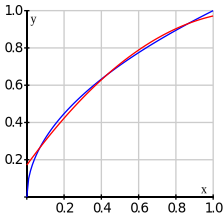
\includegraphics{6_e_example_2}}
\end{center}
\caption{The graphs of $\sqrt{x}$ and $-\frac{4}{7}x^2 + \frac{48}{35}x + \frac{6}{35}$.}
\label{F:6_e_example_2j}
\end{figure}

\item The norm of $\proj_{\pol_2^{\perp}} \sqrt{x} = \sqrt{x} - \left(-\frac{4}{7}x^2 + \frac{48}{35}x + \frac{6}{35}\right)$ tells us how well our projection $-\frac{4}{7}x^2 + \frac{48}{35}x + \frac{6}{35}$ approximates $\sqrt{x}$. Technology shows that 
\[||\proj_{\pol_2^{\perp}} \sqrt{x}|| = \sqrt{ \langle \proj_{\pol_2^{\perp}} \sqrt{x}, \proj_{\pol_2^{\perp}} \sqrt{x}\rangle } = \frac{\sqrt{2}}{70} \approx 0.02.\]

\ea

\end{example}

\csection{Summary}
\begin{itemize}
\item The Gram-Schmidt process produces an orthogonal basis from any basis. It works as follows. Let $\{\vv_1, \vv_2, \ldots, \vv_m\}$ be a basis for a subspace $W$ of an inner product space $V$. The set $\{\vw_1$, $\vw_2$, $\vw_3$, $\ldots$, $\vw_{m}\}$ defined by
\begin{itemize}
\item $\vw_1 = \vv_1$,
\item $\vw_2 = \vv_2 - \ds \frac{\langle \vv_2, \vw_1 \rangle}{\langle \vw_1, \vw_1 \rangle} \vw_1$,
\item $\vw_3 =  \vv_3 - \ds \frac{\langle \vv_3, \vw_1 \rangle}{\langle \vw_1, \vw_1 \rangle} \vw_1 - \frac{\langle \vv_3, \vw_2 \rangle}{\langle \vw_2, \vw_2 \rangle} \vw_2$, \\
\qquad $\vdots$
\item $\vw_m = \vv_m - \ds \frac{\langle \vv_m, \vw_1 \rangle}{\langle \vw_1, \vw_1 \rangle} \vw_1 - \frac{\langle \vv_m, \vw_2 \rangle}{\langle \vw_2, \vw_2 \rangle} \vw_2 - \cdots - \frac{\langle \vv_m, \vw_{m-1} \rangle}{\langle \vw_{m-1}, \vw_{m-1} \rangle} \vw_{m-1}$.
\end{itemize}
is an orthogonal basis for $W$. Moreover,
\[\Span\{\vw_1, \vw_2, \vw_3, \ldots, \vw_{k}\} = \Span\{\vv_1,\vv_2,\vv_3, \ldots, \vv_{k}\}\]
for each $k$ between 1 and $m$.
\end{itemize}



\csection{Exercises}
\be

\item Let $V = C[0,1]$ with the inner product $\langle f(t), g(t) \rangle = \int_0^1 f(t) g(t) \, dt$. Let $W = \pol_2$. Note that $W$ is a subspace of $V$. 
	\ba
	\item Find the polynomial $q(t)$ in $W$ that is closest to the function $h$ defined by $h(t) = \frac{2}{1+t^2}$ in the least squares sense. That is, find the projection of $h(t)$ onto $W$. (Hint: Recall the work done in Activity \ref{act:6_d_gs_examples}.) 
	
	\item Find the second order Taylor polynomial $P_2(t)$ for $h(t)$ centered at 0. 

	\item Plot $h(t)$, $q(t)$, and $P_2(t)$ on the same set of axes. Which approximation provides a better fit to $h$ on this interval. Why?
	
	\ea
	
\item Each set $S$ is linearly independent. Use the Gram-Schmidt process to create an orthogonal set of vectors with the same span as $S$. Then find an orthonormal basis for the same span. 
	\ba
	\item $S = \{1+t, 1-t, t-t^2\}$ in $\pol_2$ using the inner product 
\[\langle p(t), q(t) \rangle = \int_{-1}^1 p(t) q(t) \, dt\]

	\item $S = \left\{\left[ \begin{array}{c} 1\\0\\2 \end{array} \right], \left[ \begin{array}{r} -1\\1\\1 \end{array} \right], \left[ \begin{array}{c} 1\\1\\0 \end{array} \right] \right\}$ in $\R^3$ using the inner product $\langle \vu, \vv \rangle = (A\vu) \cdot (A\vv)$, where $A = \left[ \begin{array}{ccc} 1&0&1 \\ 0&1&1\\1&1&0 \end{array} \right]$

	\item $S = \left\{\left[ \begin{array}{c} 1\\0\\1\\0\\1\\0\\1 \end{array} \right], \left[ \begin{array}{r} -1\\2\\3\\0\\1\\0\\1 \end{array} \right], \left[ \begin{array}{r} 1\\0\\4\\-1\\2\\0\\1 \end{array} \right], \left[ \begin{array}{c} 1\\1\\1\\1\\1\\1\\1 \end{array} \right]\right\}$ in $\R^7$ with the weighted inner product 
\begin{align*}
 \langle [u_1 \ &u_2 \ u_3 \ u_4 \ u_5 \ u_6 \ u_7]^{\tr}, [v_1 \ v_2 \ v_3 \ v_4 \ v_5 \ v_6 \ v_7]^{\tr} \rangle \\
	&= u_1v_1 + u_2v_2 + u_3v_3 + 2u_4v_4 + 2u_5v_5 + u_6v_6 + u_7v_7
\end{align*}

	\ea

\item Let $S = \{1, \cos(t), \sin(t)\}$. 
	\ba
	\item Show that $S$ is a linearly independent set in $C[0,\pi]$.
	\item Use the Gram-Schmidt process to find an orthogonal basis from $S$ using the inner product 
	\[\langle f(t), g(t) \rangle = \int_{0}^{\pi} f(t) g(t) \, dt\]
	\ea

\item Find an orthonormal basis for the subspace $W$ of $\pol_2$ that consists of all polynomials of the form $a + (a+b)t + bt^2$ using the inner product $\langle p(t), q(t) \rangle = \int_0^1 p(t)q(t) \, dt$. 

\item The Legendre polynomials form an orthonormal basis for the infinite dimensional inner product space $\pol$ of all polynomials using the inner product 
\[\langle p(t), q(t) \rangle = \int_{-1}^{1} p(t) q(t) \, dt.\] 
The Legendre polynomials have applications to differential equations, statistics, numerical analysis, and physics (e.g., they appear when solving Schr�dinger equation in three dimensions for a central force). The Legendre polynomials are found by using the Gram-Schmidt process to find an orthogonal basis from the standard basis $\{1, t, t^2, \cdots\}$ for $\pol$. Find the first four Legendre polynomials by creating a orthonormal basis from the set $\{1,t,t^2, t^3\}$. 

\newcommand{\Si}{\text{Si}} 
\item The sine integral function $\Si$ has applications in physics and engineering. We define $\Si$ as
\[\Si(x) = \int_0^x \frac{\sin(t)}{t} \, dt.\]
Since we cannot find an elementary formula for $\Si(x)$, we use approximations. Find the best approximation to $\Si(x)$ in $\pol_3$ with inner product $\langle p(t), q(t) \rangle = \int_0^1 p(t)q(t) \, dt$. Use appropriate technology for computations and round output six places to the right of the decimal.

\item Recall from Exercise \ref{ex_6_c_all_ips} in Section \ref{sec:inner_products} that any finite dimensional vector space $V$ can be made into an inner product space by setting a basis $\CB$ for $V$ and defining
\begin{equation} \label{ex:6_e_ip}
\langle \vu, \vw \rangle_{\CB} = \sum_{i=1}^n u_iw_i 
\end{equation} 
if $\vu = \sum_{i=1}^n u_i \vv_i$ and $\vw = \sum_{i=1}^n w_i \vv_i$ in $V$. Let  $V = \pol_2$ and $\CB = \{1+t, 1+t^2, t+t^2\}$. (You may assume that $\CB$ is a basis for $V$.)
\ba
	\item Find an orthogonal basis for $V$ containing the polynomial $p_1(t) = 1$ using the inner product (\ref{ex:6_e_ip}). 
 
 \item Find the best approximation possible as measured by the inner product (\ref{ex:6_e_ip}) to the polynomial $1 + 2t + 3t^2$ by a polynomial in $\pol_1$.
	 
 \ea

\item Let $a$, $b$, and $c$ be three distinct fixed real numbers and define $\langle \ , \ \rangle : \pol_2 \to \R$ by
 \begin{equation} \label{eq:ip}
 \langle p(t),q(t) \rangle = p(a)q(a) + p(b)q(b) + p(c)q(c).
 \end{equation}
 \ba
 \item Show that $\langle \ , \ \rangle$ as defined in (\ref{eq:ip}) is an inner product on $\pol_2$.
 
\item Is the mapping 
 \begin{equation} \label{eq:ip_2}
 \langle p(t),q(t) \rangle = p(a)q(a) + p(b)q(b)
 \end{equation}
 an inner product on $\pol_2$? Justify your answer. 
 
 \item Let $a = -1$, $b=1$, and $c=3$. Find an orthogonal basis for $\pol_2$ using the inner product (\ref{eq:ip}).  
 
 \item Continue with $a = -1$, $b=1$, and $c=3$. Find the best approximation possible as measured by the inner product (\ref{eq:ip}) to the polynomial $1 + 2t + 3t^2$ by a polynomial in $\pol_1$.
 
 \item If $W = \Span\{1+t\}$, find $W^{\perp}$ in $\pol_2$ with respect to the inner product (\ref{eq:ip}). 
 
 \ea

\item Label each of the following statements as True or False. Provide justification for your response. Throughout, let $V$ be a vector space. 
	\ba
	\item \textbf{True/False} If $\{\vw_1, \vw_2\}$ is a basis for a subspace $W$ of an inner product space $V$, then the vector $\frac{\vv \cdot \vw_1}{\vw_1 \cdot \vw_1} \vw_1 + \frac{\vv \cdot \vw_2}{\vw_2 \cdot \vw_2}  \vw_2$ is the vector in $W$ closest to $\vv$. 
	\item \textbf{True/False}  If $W$ is a subspace of an inner product space $V$, then the vector $\vv - \proj_{W} \vv$ is orthogonal to every vector in $W$.
	\item \textbf{True/False} If $\vu_1$, $\vu_2$, $\vu_3$ are vectors in an inner product space $V$, then the Gram-Schmidt process constructs an orthogonal set of vectors $\{\vv_1, \vv_2, \vv_3\}$ with the same span as $\{\vu_1, \vu_2, \vu_3\}$. 
	\item \textbf{True/False} Any set $\{\vu_1, \vu_2, \ldots, \vu_k\}$ of orthogonal vectors in an inner product space $V$ can be extended to an orthogonal basis of $V$. 
	\item \textbf{True/False} Every nontrivial finite dimensional subspace of an inner product space has an orthogonal basis. 
	\item \textbf{True/False} In any inner product space $V$, if $W$ is a subspace satisfying $W^\perp=\{\vzero\}$, then $W=V$. 
	 \ea

\ee

\csection{Project: Gaussian Quadrature and Legendre Polynomials}

Simpson's rule is a reasonably accurate method for approximating definite integrals since it  models the integrand on subintervals with quadratics. For that reason, Simpson's rule provides exact values for integrals of all polynomials of degree less than or equal to 2. In Gaussian quadrature, we will use a family of polynomials to determine points at which to evaluate an integral of the form $\int_{-1}^1 f(t) \ dt$. By allowing ourselves to select evaluation points that are not uniformly distributed across the interval of integration, we will be able to approximate our integrals much more efficiently. The method is constructed so as to obtain exact values for as large of degree polynomial integrands as possible. As a result, if we can approximate our integrand well with polynomials, we can obtain very good approximations with Gaussian quadrature with minimal effort.

The Gaussian quadrature\index{Gaussian quadrature} approximation has the form
\begin{equation}
\int_{-1}^1 f(t) \ dt \approx w_1f(t_1) + w_2 f(t_2) + \cdots + w_n f(t_n) = \sum_{i=1}^n w_if(t_i), \label{eq:GQ}
\end{equation}
where the $w_i$ (weights) and the $t_i$ (nodes) are points in the interval $[-1,1]$\footnote{As we will see later, integrations over $[a,b]$ can be converted to an integral over $[-1,1]$ with a change of variable.}. Gaussian quadrature describes how to find the weights and the points in (\ref{eq:GQ}) to obtain suitable approximations. We begin to explore Gaussian quadrature with the simplest cases.

\begin{pactivity} \label{act:GQ_1} In this activity we find through direct calculation the node and weight with $n=1$ so that
\begin{equation}
w_1f(t_1) \approx \int_{-1}^1 f(t) \ dt. \label{eq:GQ1}
\end{equation}
There are two unknowns in this situation ($w_1$ and $t_1$) and so we will need 2 equations to find these unknowns. Keep in mind that we want to have the approximation (\ref{eq:GQ1}) be exact for as large of degree polynomials as possible.
	\ba
	\item Assume equality in (\ref{eq:GQ1}) if we choose $f(t) = 1$. Use the resulting equation to find $w_1$.
	

	\item Assume equality in (\ref{eq:GQ1}) if we choose $f(t) = t$. Use the resulting equation to find $t_1$.

	
	\item Verify that (\ref{eq:GQ1}) is in fact an equality for any linear polynomial of the form $f(t) = a_0+a_1t$, using the values of $w_1$ and $t_1$ you found
	
	\ea
\end{pactivity}

We do one more specific case before considering the general case.


\begin{pactivity} \label{act:GQ_2} In this problem we find through direct calculation the nodes and weights with $n=2$ so that
\begin{equation}
w_1f(t_1) + w_2f(t_2) \approx \int_{-1}^1 f(t) \ dt. \label{eq:GQ2}
\end{equation}
There are four unknowns in this situation ($w_1, w_2$ and $t_1, t_2$) and so we will need 4 equations to find these unknowns. Keep in mind that we want to have the approximation (\ref{eq:GQ2}) be exact for as large of degree polynomials as possible. In this case we will use $f(t)=1$, $f(t)=t$, $f(t)=t^2$, and $f(t)=t^3$.
	\ba
	\item Assume equality in (\ref{eq:GQ2}) if we choose $f(t) = 1$. This gives us an equation in $w_1$ and $w_2$. Find this equation.
	

	\item Assume equality in (\ref{eq:GQ2}) if we choose $f(t) = t$. This gives us an equation in $w_1, w_2$ and $t_1,t_2$. Find this equation.
	

	\item Assume equality in (\ref{eq:GQ2}) if we choose $f(t) = t^2$. This gives us an equation in $w_1, w_2$ and $t_1,t_2$. Find this equation.
	
	\item Assume equality in (\ref{eq:GQ2}) if we choose $f(t) = t^3$. This gives us an equation in $w_1, w_2$ and $t_1,t_2$. Find this equation.
	
	\item Solve this system of 4 equations in 4 unknowns. You can do this by hand or with any other appropriate tool. Show that $t_1$ and $t_2$ are the roots of the polynomial $t^2 - \frac{1}{3}$.
	
	\item Verify that (\ref{eq:GQ2}) is in fact an equality with the values of $w_1, w_2$ and $t_1, t_2$ you found for any polynomial of the form $f(t) = a_0+a_1t+a_2t^2 + a_3t^3$.

	\ea

\end{pactivity}

Other than solving a system of linear equations as in Project Activity \ref{act:GQ_2}, it might be reasonable to ask what the connection is between Gaussian quadrature and linear algebra. We explore that connection now.

In the general case, we want to find the weights and nodes to make the approximation exact for as large degree polynomials as possible. We have $2n$ unknowns $w_1$, $w_2$, $\ldots$, $w_n$ and $t_1$, $t_2$, $\ldots$, $t_n$, so we need to impose $2n$ conditions to determine the unknowns. We will require equality for the $2n$ functions $t^i$ for $i$ from 0 to $2n-1$. This yields the equations
\begin{align*}
w_1\cdot 1 + w_2\cdot 1 + \cdots + w_n\cdot 1 &= \int_{-1}^1 1 \ dt = t\biggm|_{-1}^1 = 2 \\
w_1t_1 + w_2t_2 + \cdots + w_nt_n &= \int_{-1}^1 t \ dt = \frac{t^2}{2}\biggm|_{-1}^1 = 0 \\
w_1t_1^2 + w_2t_2^2 + \cdots + w_nt_n^2 &= \int_{-1}^1 t^2 \ dt = \frac{t^3}{3}\biggm|_{-1}^1 = \frac{2}{3} \\
\qquad \vdots & \qquad \vdots \\
w_1t_1^{2n-1} + w_2t_2^{2n-1} + \cdots + w_nt_n^{2n-1} &= \int_{-1}^1 t^{2n-1} \ dt = \frac{t^{2n}}{2n}\biggm|_{-1}^1 = 0.
\end{align*}
In the $i$th equation the right hand side is
\[\int_{-1}^1 t^i \ dt = \frac{t^{i+1}}{i+1}\biggm|_{-1}^1 = \begin{cases}
\frac{2}{i+1} & \text{ if $i$ is even}, \\
0			& \text{ if $i$ is odd}.
\end{cases}\]

\begin{pactivity} \label{act:GQ_n} It is inefficient to always solve these systems of equations to find the nodes and weights, especially since there is a more elegant way to find the nodes.
	\ba
	\item Use appropriate technology to find the equations satisfied by the $t_i$ for $n=3$, $n=4$, and $n=5$. 


	\item Now we will see the more elegant way to find the nodes. As we will show for some cases, the nodes can be found as roots of a set of orthogonal polynomials in $\pol_n$ with the inner product $\langle f(t), g(t) \rangle = \int_{-1}^1 f(t)g(t) \ dt$. Begin with the basis $\CS_n = \{1, t, t^2, \ldots, t^n\}$ of $\pol_n$. Use appropriate technology to find an orthogonal basis $B_5$ for $\pol_5$ obtained by applying the Gram-Schmidt process to $\CS_n$. The polynomials in this basis are called \emph{Legendre polynomials}. Check that the nodes are roots of the Legendre polynomials by finding roots of these polynomials using any method. Explain why the $t_i$ appear to be roots of the Legendre polynomials.
				
	\ea
\end{pactivity}

Although it would take us beyond the scope of this project to verify this fact, the nodes in the $n$th Gaussian quadrature approximation (\ref{eq:GQ}) are in fact the roots of the $n$th order Legendre polynomial. In other words, if $p_n(t)$ is the $n$th order Legendre polynomial, then $t_1$, $t_2$, $\ldots$, $t_n$ are the roots of $p_n(t)$ in $[-1,1]$. Gaussian quadrature as described in (\ref{eq:GQ}) using the polynomial $p_n(t)$ is exact if the integrand $f(t)$ is a polynomial of degree less than $2n$.

We can find the corresponding weights, $w_i$, using the formula\footnote{Abramowitz, Milton; Stegun, Irene A., eds. (1972), �25.4, Integration, Handbook of Mathematical Functions (with Formulas, Graphs, and Mathematical Tables), Dover,}
\begin{equation}
w_i = \frac{2}{(1-t_i^2)(q_n '(t_i))^2}, \label{eq:GQ_weights}
\end{equation}
where $q_i(t)$ is the $i$th order Legendre polynomial scaled so that $q_i(1)=1$.

\begin{pactivity} \label{act:GQ_example} Let us see now how good the integral estimates are with Gaussian quadrature method using an example. Use Gaussian quadrature with the indicated value of $n$ to approximate $\displaystyle \int_{-1}^1 e^t\cos(t) \ dt$. Be sure to explain how you found your nodes and weights (approximate the nodes and weights to 8 decimal places). Compare the approximations with the actual value of the integral. Use technology as appropriate to help with calculations. 
	\ba
	\item $n=3$
		
	\item $n=4$
	
	\item $n=5$
	

	\ea


\end{pactivity}

Our Gaussian quadrature formula was derived for integrals on the interval $[-1,1]$. We conclude by seeing how a definite integral on an interval can be converted to one on the interval $[-1,1]$.  

\begin{pactivity} Consider the problem of approximating an integral of the form $I = \int_a^b g(x) \ dx$.  Show that the change of variables $x = \frac{(b - a)t}{2} + \frac{a + b}{2}$, $f(t) = \frac{(b - a)g(x)}{2}$ reduces the integral $I$ to the form $I = \int_{-1}^1 f(t) \ dt$.  (This change of variables can be derived by finding a linear function that maps the interval $[a,b]$ to the interval $[-1,1]$.) 


\end{pactivity}

